\section{系统设计}

\subsection{系统总体设计}

本系统的整体架构采用Django的MVT三层设计模式,其中M表示Model层、V表示View层以及T表示Template层。从工厂信息管理着手,如图\ref{fig:sysarc}所示,首先对系统总体功能进行设计,选择开发环境以及数据库,之后对数据层进行功能设计,例如事务管理以及读写数据库等,然后设计业务层的业务逻辑,例如交易信息管理、员工信息管理和人脸识别签到等,之后使用模板渲染对前端页面进行后端数据的渲染,最后向用户展示。

\begin{figure}[H]
    \centering
    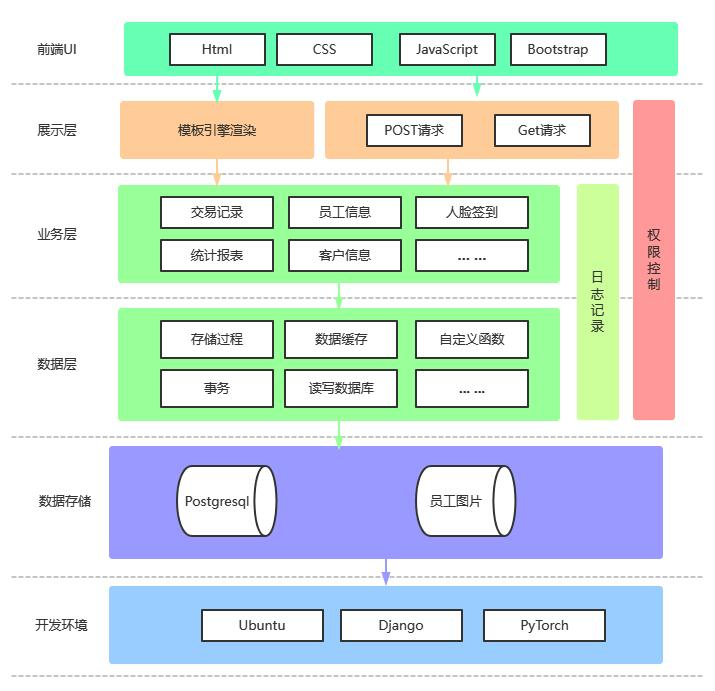
\includegraphics[width=.75\textwidth]{figures/4total.jpg}
    \caption{系统架构图}
    \label{fig:sysarc}
\end{figure}

